%%% result.tex 
%% displays experimental setup, and description of matrices 
We performed a series of experiments to test robustness and overhead of our algorithm described in~\refsec{sec:connected}. 

%
\subsection{Fault Injection Methodology}
Since memory accesses are most performance critical part in~\sv computation, we inject faults in memory access pattern. There are two main memory accesses in~\sv iteration: traversing adjacency list for each vertex; and 
accessing $CC$ array for each vertex in adjacency list. 

In the first case, before each~\sv sweep, we randomly select $f|E|$ edges, where $f$ is fault-rate. Let $e=(v,u)$ be  one of the selected edges. When we encounter $e$ while traversing adjacency list of $v$, we flip one of the bits of $u$---the vertex which $e$ is pointing---randomly. 
Therefore, due to the fault, $v$ will visit flipped vertex $\hat{u}$, instead of accessing $u$. 

In the second case, we will again choose another set of $f|E|$ edges. Let $e=(v,u)$ be  one of the selected edges. When we encounter $e$ while traversing adjacency list of $v$, we flip one of the bits of $CC[u]$.
Therefore, due to the fault, $v$ will visit the correct vertex, however, it see incorrect value of  $CC[u]$.
It should be noted that $CC[u]$ will be accessed multiple times in a~\sv iteration, and we assume that 
all accesses to $CC[u]$ in an iteration are independent. In other words, if $CC[u]$ is accesses while visiting 
vertex $v_{1},\ v_{2}$, and if $CC[u]$ is corrupted while visiting $v_{1}$, then $CC[u]$ may or may not be corrupted when it is accessed while visiting $v_{2}$.


\subsection{Experimental Setup}



% type of matrices 
\paragraph{Test Graphs}
The graphs used in our tests are listed in~\reftab{tab:graphs}. 
These graphs are taken from the 10th Dimacs Implementation Challenge~\cite{Bader-dimacs-graph2014}, come from various real and synthetic applications. 
\begin{table*}[ht]
\ra{1.3}
\centering
\caption{List of matrices used for experimentation}
\label{tab:graphs}
\begin{tabular}{l|llll}
\toprule 
Matrix Name              & Source                          & \#Vertices & \#Edges  & $|E|/|V|$ \\
\midrule 
astro-ph                 & collaboration network           & 16706      & 242502   & 14.5      \\
audikw1                  & UF Sparse Matrix Collection     & 943695     & 77651847 & 82.3      \\
caidaRouterLevel         & Internet router-level graph     & 192244     & 1218132  & 6.3       \\
cnr-2000                 & Web crawl                       & 325557     & 2738969  & 8.4       \\
citationCiteseer         & Citation network                & 268495     & 1156647  & 4.3       \\
coAuthorsDBLP            & Citation network                & 299067     & 977676   & 3.3       \\
coPapersDBLP             & Citation network                & 540486     & 15245729 & 28.2      \\
cond-mat-2005            & Condensed matter collaborations & 40421      & 175691   & 4.32      \\
delaunay\_n18            & Delaunay triangulations         & 262144     & 786396   & 3.0       \\
er-fact1.5-scale20       & Erdos-Renyi Graphs              & 1048576    & 10904496 & 10.4      \\
G\_n\_pin\_pout          & Gnp random-graph                & 100000     & 501198   & 5.01      \\
kron\_g500-simple-logn18 & synthetic graphs                & 262144     & 10582686 & 40.4      \\
ldoor                    & Sparse Matrix                   & 952203     & 22785136 & 24        \\
preferentialAttachment   & Clustering Instances            & 100000     & 499985   & 5         \\
rgg\_n\_2\_18\_s0        & random geometric graph          & 262144     & 1547283  & 5.9      \\

\bottomrule 
\end{tabular}
\end{table*}

\paragraph{Testbed}
\begin{table}[]
\centering
\caption{Testbeds used for performance evaluation.}
\label{tab:sys_info}
\begin{tabular}{ll}
Prop                 & SNB20c       \\
Sockets$\times$Cores & 2$\times$8   \\
Clock Rate           & 2.4GHz       \\
DRAM capacity        & 128GB        \\
DRAM Bandwidth       & 72GB/s      
\end{tabular}
\end{table}
We prototyped baseline and fault tolerant implementation using $C$ language. 
We used the Intel C Compiler (ICC 15.0.0), with highest level of
 optimization $-O3$ to compile our benchmarks.
We ran all our experiments on SNB16c, key properties of the systems are listed in~\reftab{tab:sys_info}


\subsection{Convergence in presence of faults}

\begin{figure}[tbp]
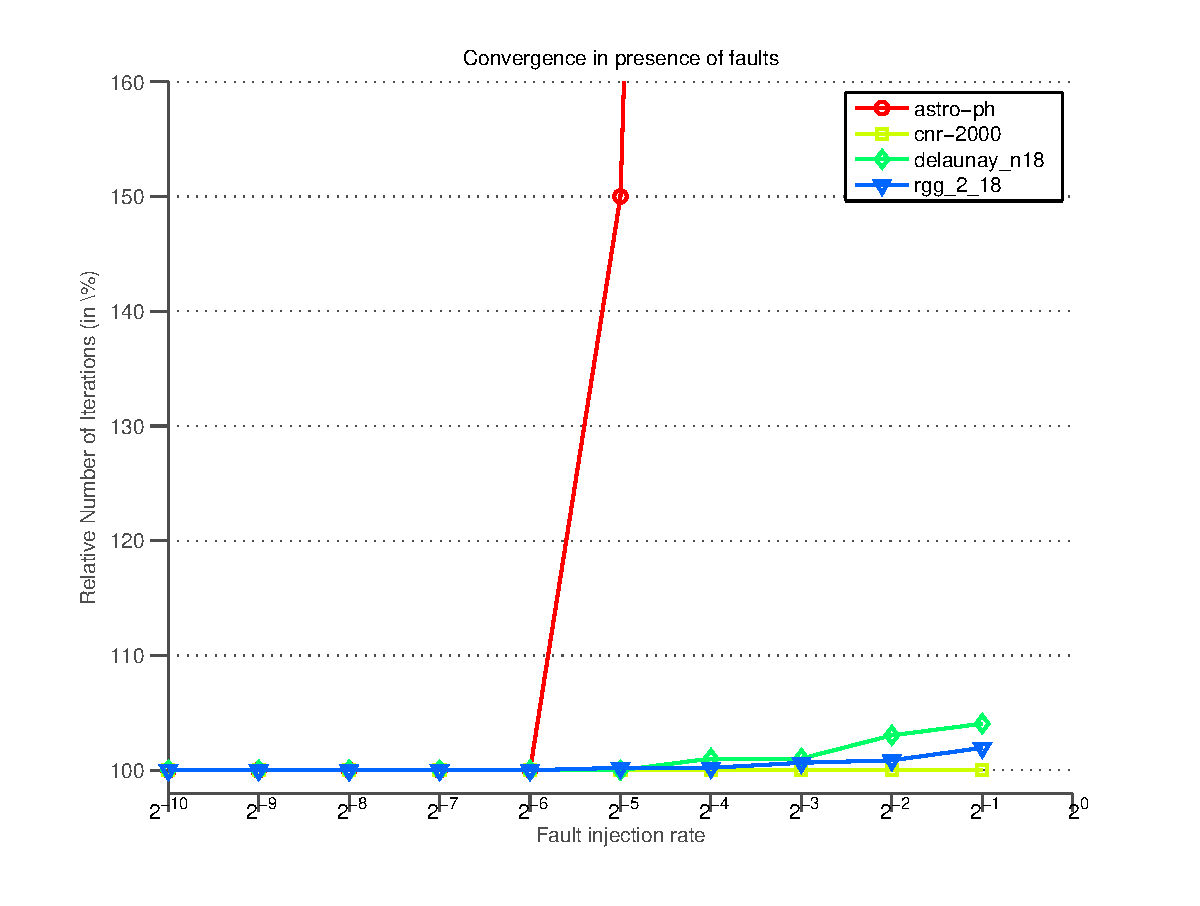
\includegraphics[width=.5\textwidth]{plots/plot_conv.eps}
\caption{\label{fig:con-plot} 
\small Comparison of model-driven work partitioning scheme to
two static work partitioning scheme}
\end{figure}

First, we try to understand the convergence property of~\sv algorithm 
in presence of faults. 
Recall that in the worst case, an \emph{acceptable} fault that is not detected by~\refalg{alg:FTSV_ALG}, may delay the convergence by one iteration. On the other hand, one additional iteration means additional faults, which may necessitate an additional iteration for convergence. 
Thus, it is expected that with increasing fault rate, convergence might slow down. To understand practicality of our algorithm, it becomes essential to understand such slow down in convergence.  

% what do we do
In~\reffig{fig:con-plot}, we show the convergence of \sv~algorithm in presence of faults for four graphs. We vary the fault rate from $2^-{10} \times |E|$ bit flips in every~{\sv}~ iteration to $2^-{1} \times |E|$ bit flips. Note that this fault injection rate is extremely high and, we do so to stress test the proposed algorithm.

%what do we observe
In~\reffig{fig:con-plot}, we observe that for all practical fault rates($<2^{-6}|E|$) , algorithm converges without any additional iteration.
Additionally, except~\graphname{astro-ph}, all other graphs converge to correct solution within 5\% additional iteration at the highest fault rate. As such, we conclude that our proposed algorithm can withstand high fault rates, with minimal additional iteration overhead.   

% why do we observe that
The difference in behavior between graph~\graphname{astro-ph}, and other graphs is due to two reasons. First, the graph~\graphname{astro-ph} has  the smallest diameter all four test cases, and it only takes 10 iterations in fault free case to converge. If a fault that might cause an additional iteration occurs, it provides fewer opportunity to be corrected in later iterations. Secondly, ...

\subsection{Overhead of fault detection and correction}
%% compare it with double modular redundancy 

